\section{Measuring reactive components} \label{sec:MeasureReactiveComponents}
Impedance is the magnitude and phase angle between voltage and current, and thus to measure impedance, both voltage and current must be measured together with
their phase difference. From this it follows that to characterize the impedance of a device, voltage, current and their phase must be measured. An LCR meter measures exactly these parameters
at the desired test frequency, LCR meters, unlike oscilloscopes and signal generators, are however not a common laboratory instrument. The authors of this document are both
electronics technicians and testify to the quote "It is not always easy to find an LCR meter" from Tektronix \Cite{TektronixZMeas}. 

To measure the impedance of a component, an oscilloscope, signal generator and precision resistor can however be used as an alternative to an LCR meter. Such a setup is illustrated in figure \ref{fig:Prob:HowItWorks:ImpedanceMeas}, where a signal generator is used to excite the unknown device, and a reference ressitor is used as a shunt to measure the current. An oscilloscope is then used to measure both the amplitude and phase of voltage and current. 

\begin{figure}[H]
    \centering
    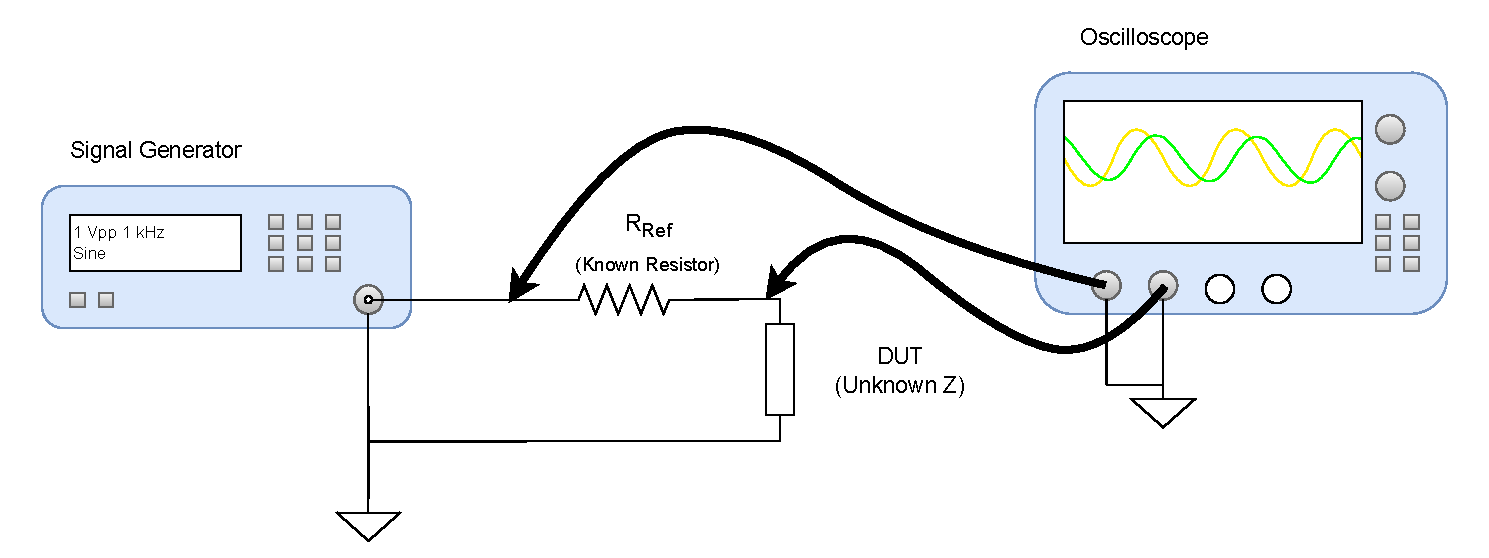
\includegraphics[width=1\textwidth]{Sections/2_ProblemAnalysis/Figures/ScopeGenZMeas.pdf}
    \caption{Impedance measurement with an oscilloscope and signal generator.}
    \label{fig:Prob:HowItWorks:ImpedanceMeas}
\end{figure}